\documentclass{standalone}

\usepackage{tikz}
\usepackage{amssymb}
\usetikzlibrary{calc, positioning}
\begin{document}
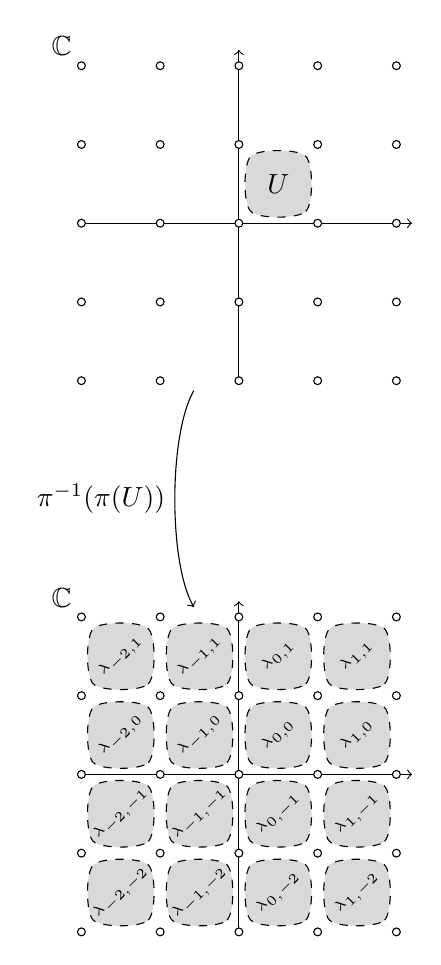
\begin{tikzpicture}
  \draw[->] (-2,0) to (2.2,0);
  \draw[->] (0,-2) to (0,2.2);
  \foreach \x in {-2,-1,...,2} {
    \foreach \y in {-2,-1,...,2} {
      \filldraw[fill=white] (\x, \y) circle[radius=0.05];
    };
  };
\filldraw[dashed, fill=gray!50, fill opacity=0.6] plot[smooth cycle]
  coordinates{(0.15,0.15) (0.85,0.15) (0.85,0.85) (0.15,0.85)};
  \node at (0.5,0.5) {$ U $}; 
  \node[above left] at (-2,2) {$ \mathbb{C} $};
  \node (l) at (-0.5,-2){};

\begin{scope}[yshift=-7cm]
  \draw[->] (-2,0) to (2.2,0);
  \draw[->] (0,-2) to (0,2.2);
  \foreach \x in {-2,-1,...,2} {
    \foreach \y in {-2,-1,...,2} {
      \filldraw[fill=white] (\x, \y) circle[radius=0.05];
    };
  };

\foreach \x in {-2,-1,...,1} {
  \foreach \y in {-2,-1,...,1} {
    \begin{scope}[yshift=\y cm, xshift=\x cm]
      \filldraw[dashed, fill=gray!50, fill opacity=0.6] plot[smooth cycle]
        coordinates{(0.15,0.15) (0.85,0.15) (0.85,0.85) (0.15,0.85)};
      \node[rotate=45] at (0.5,0.5) {\tiny$ \lambda _{\x, \y} $}; 
    \end{scope}
  };
};

  \node (r) at (-0.5,2){};
  \node[above left] at (-2,2) {$ \mathbb{C} $};
\end{scope}

\draw[->, bend right, looseness=0.6] (l) to node[left]{$ \pi ^{-1}(\pi(U)) $} (r);
\end{tikzpicture}
\end{document}
